
\renewcommand{\resultsfigwidth}{1.27in}
\renewcommand{\resultscropwidth}{0.84in}
% \renewcommand{\resultscropwidth}{0.79in}

% Define the crops here, individually for each image
\newcommand{\cropfern}[1]{
  \makecell{
  % left bottom right top
%   \includegraphics[trim={84px 328px 794px 298px}, clip, width=\resultscropwidth]{#1} \\
%   \includegraphics[trim={174px 178px 654px 398px}, clip, width=\resultscropwidth]{#1} \\
%   \includegraphics[trim={826px 164px 14px 424px}, clip, width=\resultscropwidth]{#1} 
%   \includegraphics[trim={704px 448px 204px 208px}, clip, width=\resultscropwidth]{#1} 
  \includegraphics[trim={774px 178px 54px 398px}, clip, width=\resultscropwidth]{#1} \\
  \includegraphics[trim={93px 339px 801px 303px}, clip, width=\resultscropwidth]{#1} 
  }
}

\newcommand{\croporchid}[1]{
  \makecell{
  % left bottom right top
%   \includegraphics[trim={4px 328px 874px 298px}, clip, width=\resultscropwidth]{#1} \\
%   \includegraphics[trim={204px 428px 704px 228px}, clip, width=\resultscropwidth]{#1} \\
%   \includegraphics[trim={624px 438px 204px 138px}, clip, width=\resultscropwidth]{#1} \\
%   \includegraphics[trim={504px 428px 404px 228px}, clip, width=\resultscropwidth]{#1} \\
%   \includegraphics[trim={624px 438px 204px 138px}, clip, width=\resultscropwidth]{#1} \\
  \includegraphics[trim={205px 404px 681px 230px}, clip, width=\resultscropwidth]{#1} \\
  \includegraphics[trim={516px 393px 364px 235px}, clip, width=\resultscropwidth]{#1} 
  }
}

% \newcommand{\cropredflower}[1]{
%   \makecell{
%   % left bottom right top
% %   \includegraphics[trim={304px 438px 574px 188px}, clip, width=\resultscropwidth]{#1} \\
%   \includegraphics[trim={424px 308px 484px 348px}, clip, width=\resultscropwidth]{#1} \\
%   \includegraphics[trim={674px 118px 174px 488px}, clip, width=\resultscropwidth]{#1}
%   }
% }

\newcommand{\cropredtrex}[1]{
  \makecell{
  % left bottom right top
%   \includegraphics[trim={484px 308px 384px 308px}, clip, width=\resultscropwidth]{#1} \\
%   \includegraphics[trim={374px 118px 474px 488px}, clip, width=\resultscropwidth]{#1} \\
%   \includegraphics[trim={584px 248px 324px 408px}, clip, width=\resultscropwidth]{#1} \\
%   \includegraphics[trim={384px 208px 484px 408px}, clip, width=\resultscropwidth]{#1} \\
%   \includegraphics[trim={184px 48px 714px 578px}, clip, width=\resultscropwidth]{#1} 
  \includegraphics[trim={384px 280px 478px 330px}, clip, width=\resultscropwidth]{#1}   \\
  \includegraphics[trim={183px 61px 715px 585px}, clip, width=\resultscropwidth]{#1} 
  }
}
% 368px 209px 492px 399px

% \setlength{\tabcolsep}{1mm}
\afterpage{\clearpage}
\begin{figure}[p]
\centering
\scriptsize
\begin{tabular}{@{}c@{\,\,}c@{}c@{}c@{}c@{}}
% \begin{tabular}{@{}c@{\,\,}c@{\,\,}c@{}c@{}c@{}c@{}}
% \begin{tabular}{ccccc}
\makecell[c]{
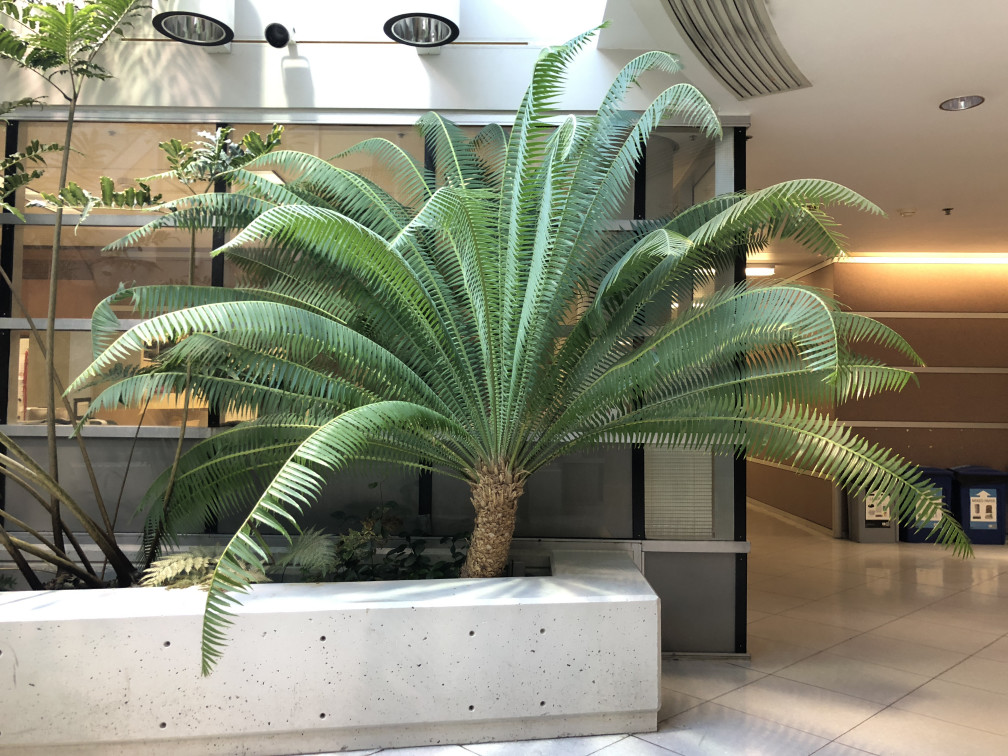
\includegraphics[trim={0px 0px 0px 0px}, clip, width=\resultsfigwidth]{figs/real_results_new/fern/gt.jpg}
\\
\scenename{Fern}
}
& 
\cropfern{figs/real_results_new/fern/gt.jpg} &
\cropfern{figs/real_results_new/fern/nerf.jpg} &
\cropfern{figs/real_results_new/fern/llff.jpg} &
\cropfern{figs/real_results_new/fern/srn.jpg} \\
\makecell[c]{
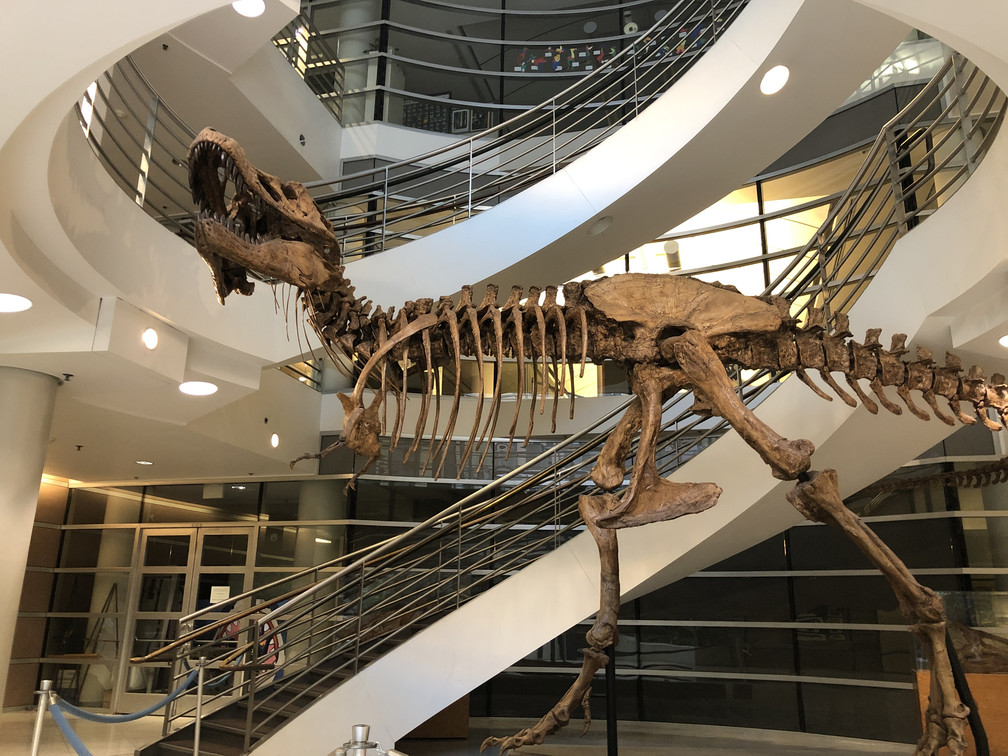
\includegraphics[trim={0px 0px 0px 0px}, clip, width=\resultsfigwidth]{figs/real_results_new/trex/gt.jpg}
\\
\scenename{T-Rex}
}
& 
\cropredtrex{figs/real_results_new/trex/gt.jpg} &
\cropredtrex{figs/real_results_new/trex/nerf.jpg} &
\cropredtrex{figs/real_results_new/trex/llff.jpg} &
\cropredtrex{figs/real_results_new/trex/srn.jpg} \\
\makecell[c]{
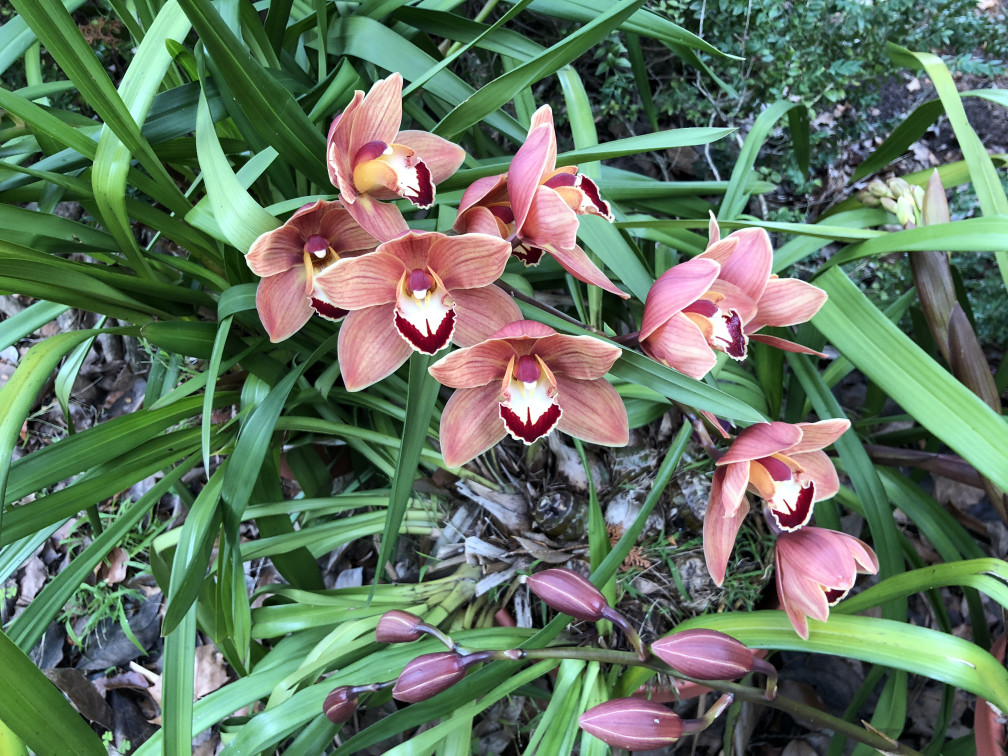
\includegraphics[trim={0px 0px 0px 0px}, clip, width=\resultsfigwidth]{figs/real_results_new/orchid/gt.jpg}
\\
\scenename{Orchid}
}
& 
\croporchid{figs/real_results_new/orchid/gt.jpg} &
\croporchid{figs/real_results_new/orchid/nerf.jpg} &
\croporchid{figs/real_results_new/orchid/llff.jpg} &
\croporchid{figs/real_results_new/orchid/srn.jpg} \\
& Ground Truth & NeRF (ours) & LLFF~\cite{mildenhall19} & SRN~\cite{srn} 
\end{tabular}
\caption{Comparisons on test-set views of real world scenes. LLFF is specifically designed for this use case (forward-facing captures of real scenes). Our method is able to represent fine geometry more consistently across rendered views than LLFF, as shown in \scenename{Fern}'s leaves and the skeleton ribs and railing in \scenename{T-rex}. Our method also correctly reconstructs partially occluded regions that LLFF struggles to render cleanly, such as the yellow shelves behind the leaves in the bottom \scenename{Fern} crop and green leaves in the background of the bottom \scenename{Orchid} crop. Blending between multiples renderings can also cause repeated edges in LLFF, as seen in the top \scenename{Orchid} crop. SRN captures the low-frequency geometry and color variation in each scene but is unable to reproduce any fine detail.
% LLFF is specifically designed for this use case (forward-facing real world captures) but still sometimes fails to consistently estimate geometry for complex objects, such as the leaf in the top \scenename{Fern} crop and the skeleton ribs and railing in \scenename{T-rex}. LLFF often struggles to cleanly render objects that are partially occluded, like the shelves in the second row and the green leaves in the last row of \scenename{Orchid}. SRN captures the low-frequency geometry and color variation of the scene but is unable to reproduce any fine detail.
}
\label{fig:realresults}
\end{figure}
